\documentclass[12pt,a4paper,bibtotocnumbered,liststotocnumbered]{scrreprt}
\usepackage[utf8x]{inputenc}
\usepackage{color}
\usepackage[german]{babel}
\usepackage[T1]{fontenc}
%\usepackage[scaled]{uarial}
\usepackage{amsmath}
\usepackage[printonlyused]{acronym}
\usepackage{amsfonts}
\usepackage{amssymb}
\usepackage{graphicx}
\usepackage{rotating}

\usepackage{float}
\setlength{\parindent}{0pt}
\usepackage{url}
\urlstyle{same}
\usepackage{enumitem}

\usepackage{pdflscape}
\usepackage[left=2cm,right=2cm,top=2cm,bottom=2cm]{geometry}
\usepackage{chemfig}
\usepackage{cancel}
\usepackage{caption}
\usepackage{mhchem}
\usepackage{svg}
\usepackage[outdir=./Grafiken/]{epstopdf}


%Tikx -----------------------------------
\usepackage{tikz}
\usetikzlibrary{arrows,arrows.meta,intersections,shapes,positioning,shadows, decorations, snakes}
% \tikzexternalize ,external 
\tikzset{%
  >={Latex[width=2mm,length=2mm]},
  % Specifications for style of nodes:
  			every node/.style={align=center, fill = white},
            base/.style = {rectangle, rounded corners, draw=black, minimum width=3cm, minimum height=1cm, text centered, font=\sffamily},
            test/.style = {rectangle, rounded corners, draw=black, text centered, minimum width=2.5cm, minimum height=1cm, font=\sffamily]},
            entscheidung/.style = {diamond, rounded corners, draw=black, text centered, minimum width=2.5cm, minimum height=1cm, font=\sffamily},
  			blue/.style = {base, fill=blue!30, very thick},
      		 red/.style = {base, fill=red!30},
  		   green/.style = {test, fill=green!30},
          orange/.style = {base, fill=orange!15},
          	bier/.style = {base, fill=yellow!30, very thick},      
             mix/.style = {base,circle, minimum width=4mm, fill=green!15},
    }
    
\def\checkmark{\tikz\fill[scale=0.4](0,.35) -- (.25,0) -- (1,.7) -- (.25,.15) -- cycle;} 


%\color{
\definecolor{lightgray}{gray}{0.95}
\definecolor{latex}{rgb}{0,0.2,0.4}
\definecolor{befehle}{rgb}{0.55,0,0}
\definecolor{orange}{rgb}{1,0.41,0.13}
%}

%\color[rgb]{1,1,0.88}




%NatBib
\usepackage[square,numbers]{natbib}
\bibliographystyle{unsrt}
\usepackage{ragged2e}

%-------------------------------------------
%\fancypagestyle{plain}{ %
%  \fancyhf{} % remove everything
%  \renewcommand{\headrulewidth}{0pt} % remove lines as well
%  \renewcommand{\footrulewidth}{0pt}
%}


\usepackage{fancyhdr}


\renewcommand{\rmdefault}{ptm}
\newcommand{\underlined}[1]{\underline{\underline{#1}}}

%--------------------------------------------------------------------------
%Einheitenimplementierung
\usepackage{siunitx}
\sisetup{
  locale = US,
  per-mode = symbol,
  overwrite-functions = true
}

\NewDocumentCommand\DeclareNewQuantity{mmm}{
  \DeclareSIUnit{#1}{#3}
  \DeclareDocumentCommand{#2}{O{}m}{\SI[##1]{##2}{#1}}
}

%\newcommand{\tief}[1]{_{\, \mathsf{#1}}}
%\newcommand{\R}{\SI{8,314}{\kilo\gram\square\meter\per\square\second\per\mol\per\kelvin}}
\newcommand{\note}[1]{(\textit{\textbf{Anmerkung:} #1})}



\DeclareNewQuantity{\helpa}{\dichte}{\gram\per\cubic\centi\meter}
\DeclareNewQuantity{\helpb}{\Dichte}{\kilo\gram\per\cubic\meter}
\DeclareNewQuantity{\helpc}{\speed}{\meter\per\second}
\DeclareNewQuantity{\helpd}{\accel}{\meter\per\square\second}
%\DeclareNewQuantity{\helpe}{}{}
%\DeclareNewQuantity{\helpf}{}{}
%\DeclareNewQuantity{\helpg}{}{}
%\DeclareNewQuantity{\helph}{}{}
%\DeclareNewQuantity{\helpi}{}{}
%\DeclareNewQuantity{\helpj}{}{}
%\DeclareNewQuantity{\helpk}{}{}
%\DeclareNewQuantity{\helpl}{}{}
%\DeclareNewQuantity{\helpm}{}{}
%\DeclareNewQuantity{\helpn}{}{}
%\DeclareNewQuantity{\helpo}{}{}
%\DeclareNewQuantity{\helpp}{}{}





%-------------------------------------------------------------------------

\definecolor{Grau}{gray}{0.5}

\definecolor{lightblue}{RGB}{80,100,200}
\definecolor{lightgreen}{RGB}{200,255,200}
\definecolor{lightgray}{RGB}{200,200,200}
\definecolor{lightred}{RGB}{255,200,200}
\definecolor{lightyellow}{RGB}{255,255,200}

\transparent{0.5}
\newcommand{\green}[1]{\colorbox{lightgreen}{$\displaystyle #1$}}
\newcommand{\black}[1]{\colorbox{lightgray}{$\displaystyle #1$}}
\newcommand{\red}[1]{\colorbox{lightred}{$\displaystyle #1$}}
\newcommand{\yellow}[1]{\colorbox{lightyellow}{$\displaystyle #1$}}




%------------------------------------------------------------------------
\usepackage{Style/classic_style}

\mgrad{Master of Science}
\institution[OVGU Magdeburg]{Otto-von-Guericke-Universität Magdeburg}
\logo{Logo.eps}
\title{\textbf{Luftfilteranlagen zur Reinigung von Raumluft}\\zur Bekämpfung der Ausbreitung des Corona Virus in geschlossenen Räumen}
\author{Florian Jacob \\Kontakt: \url{florian.jacob@ovgu.de}}
\date{\today}



\usepackage{hyperref}

%Dokumentvariablen
\newcommand{\Konz}{n}

\begin{document}
\pagenumbering{Roman}
\maketitle
\tableofcontents
\newpage
\pagenumbering{arabic}
\plain



\chapter{Bisherige Forschungsergebnisse}

\chapter{Simulation der Partikel-Konzentration}
Um nicht in jedem Raum die Partikel-Konzentration messen zu müssen, ist es sinnvoll ein Modell zu entwickeln. Dieses kann dann in einer Simulation die Partikel-Konzentration anhand bestimmter Parameter bemessen.

\section{Theoretische Modellgrundlagen}
Für die Simulation der Viruslast gibt es mehrere relevante Einflussfaktoren. Diese lassen sich prinzipiell in 4 Gruppen einteilen:
\begin{itemize}
\item Partikel-Bildung
\item Partikel-Abbau durch den Luftreiniger
\item Partikel-Abbau durch das Fensterlüftung
\item Neutralisierung der Partikel durch das Absterben der Viren
\end{itemize}
Für jeden dieser Faktoren lassen sich nun Gleichungen bzw. Algorithmen finden, die die Entwicklung der Viruslast beschreiben.
\subsection{Bildung der Partikel}
Die Partikelbildung ist sehr stark von der Aktivität der Person abhängig. Daraus ergibt sich zum einen das Atemvolumen, zum anderen aber auch die Konzentration an Partikeln in der ausgeatmeten Luft.
\begin{align}
\dot{P}\tief{add} = c\tief{breath}\dot{V}\tief{breath}
\end{align}
Mit Hilfe der Raumgröße und der Annahme idealer Durchmischung der Raumluft lässt sich daraus die Änderung der Partikel-Konzentration bestimmen.
\begin{align}
\dot{c}\tief{add} =\frac{\dot{P}\tief{add}}{V\tief{room}}
\end{align}
Für die nicht infizierten Personen ändert sich durch die Erhöhung ihres Atemvolumens auch Signifikat ihr Infektionsrisiko.
\begin{align}
\dot{P}\tief{inhaliert} = c\tief{ges}\dot{V}\tief{breath}
\end{align}
\begin{tabular}{ll}
$\dot{P}\tief{add}$ & Durch Ausatmen eingetragener Partikelanzahlstrom (Partikel$/s$)\\
$c\tief{breath}$ & Konzentration der Partikel in der Ausatemluft (Partikel$/m^3$)\\
$\dot{V}\tief{breath}$ & Durchschnittlicher Atemvolumenstrom ($m^3/s$)\\
$\dot{c}\tief{add}$ & Durch Ausatmen erzeugte Änderung der  Raumkonzentration (Partikel$/(m^3\cdot s)$)\\
$V\tief{room}$ & Raumvolumen ($m^3$)\\
$\dot{P}\tief{inhaliert}$ & Durch Einatmen aufgenommene Partikelanzahl (Partikel$/s$)\\
\end{tabular}


\subsection{Abbau der Partikel durch den Luftreiniger}
Ein Luftreiniger saugt mithilfe eines Motors einen gewissen Luftstrom an und reinigt diesen zu einem gewissen Grad. Es lässt sich also formulieren:
\begin{align}
\dot{P}\tief{ap} &=\dot{V}\tief{ap} \eta\tief{ap} c\tief{room}\\
\dot{c}\tief{ap} &=-\frac{\dot{P}\tief{ap}}{V\tief{room}}
\end{align}
\begin{tabular}{ll}
$\dot{P}\tief{ap}$ & Durch Luftreiniger entfernte Partikelanzahl (Partikel$/s$)\\
$c\tief{room}$ & Konzentration der Partikel im Raum (Partikel$/m^3$)\\
$\dot{V}\tief{ap}$ & Durchschnittlicher Volumenstrom des Luftreinigers ($m^3/s$)\\
$\eta\tief{ap}$ & Partikel-Wirkungsgrad des Luftreinigers ($\%$)\\
$\dot{c}\tief{ap}$ & Durch Luftreiniger erzeugte Änderung der  Raumkonzentration (Partikel$/(m^3\cdot s)$)\\
\end{tabular}

\subsection{Abbau der Partikel durch Lüften}
Durch Lüften verdünnt sich quasi die Raumluft. Damit lässt sich die Partikel-Anzahl beschreiben mit:
\begin{align}
P\tief{room,t+1} = P\tief{room,t} \cdot \left( 1 -  \frac{\eta\tief{vent}}{t\tief{vent}}\right)
\end{align}
\begin{tabular}{ll}
$P\tief{room,t} $ & Partikelanzahl im Raum (Partikel)\\
$\eta\tief{vent}$ & Lüftungseffizienz (Raumvolumen/Luftaustauschstrom in Lüftungszeitraum, $s$)\\
$t\tief{vent} $ & Lüftungsdauer ($s$)\\
\end{tabular}
Das Lüften findet immer in Intervallen $t\tief{ventintervall} $ statt und wird zu den anderen Zeiten übersprungen.

\subsection{Neutralisation der Viruspartikel durch Absterben}
Um den Effekt des Absterbens zu simulieren, werden die Viruspartikel in einzelne Fraktionen mit dem entsprechenden Zeitpunkt gespeichert. Da sich die Fraktionen nur minimal gegenseitig beeinflussen, kann jede der vorherigen Operationen auch auf jede Gruppe einzeln angewendet werden. Ist eine Fraktion älter als die Viruslebensdauer $t\tief{vir}$, so wird ihre Anzahl auf 0 gesetzt. Auch ein Modell, das ein Absterben mit Hilfe einer Normalverteilung um den Todeszeitpunkt nutzt, wurde untersucht, führte jedoch zu keiner signifikanten Änderung der Ergebnisse. 

\section{Bildung einer Modellfunktion}
Die Berechnung der Konzentration der mit Virus beladenen Partikel in der Raumluft führt zu einem zeitlichen Verlauf, wie er in der blauen Kurve in \autoref{Abb: Simulation} dargestellten ist. Der zeitliche Mittelwert ist dabei eine relativ stetige Funktion, die sich möglicherweise mit einer einfacheren mathematischen Funktion approximieren lässt. Mit Hilfe einer solchen Funktion ließe sich der zeitliche Verlauf der Partikelkonzentration für verschiedene Randbedingungen wesentlich schneller bestimmen, als mit der zuvor vorgestellten Methode.
\begin{figure}[H]
\begin{center}
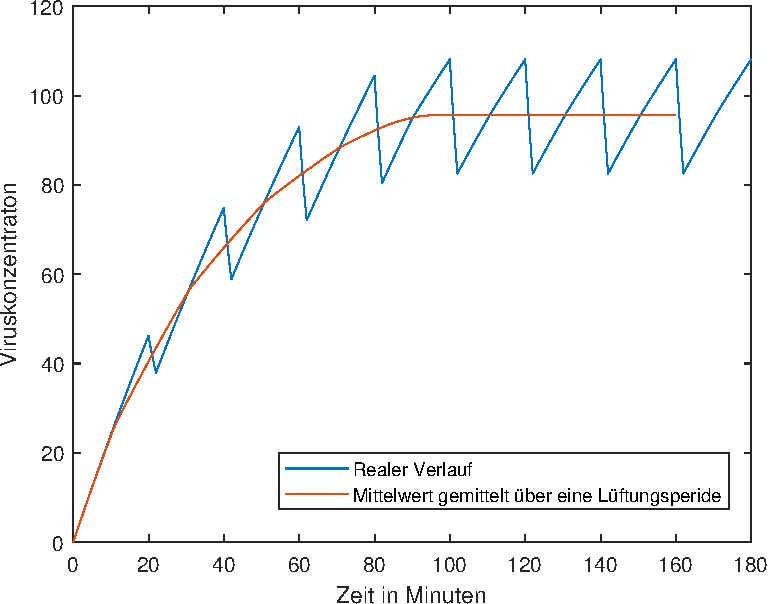
\includegraphics[width =0.8 \textwidth]{Simulation.pdf}
\caption{Entwicklung der Partikel-Konzentration im Raum}
\label{Abb: Simulation}
\end{center}
\end{figure}

Um eine potentielle Funktion zu bestimmen, ist es interessant, sich Grenzwerte anzuschauen. Dabei sind interessant:
\begin{align}
\label{Equ.: c_max}
\lim \limits_{t \to \infty} c(t) & = c\tief{max}\\
\label{Equ.: c_inf_abl}
\lim \limits_{t \to \infty} \dot{c}(t) & = 0\\
\lim \limits_{t \to 0} c(t) & = 0\\
\label{Equ.: m_0}
\lim \limits_{t \to 0} \dot{c}(t) & = m\tief{0}
\end{align}

\begin{tabular}{ll}
$c\tief{max} $ & Maximale Konzentration, Grenzwert\\
$m\tief{0}$ & Anfangsanstieg\\
\end{tabular}

Für die Bestimmung von $m\tief{0}$ lässt sich eine einfache Betrachtung anstellen. Da zu Beginn die Partikel noch nicht absterben, entspringt die Konzentrationsänderung hier nur der durch die Atemluft erzeugten Partikel ($\dot{c}\tief{add}$).\\

Eine Funktion, die die Limes Bedingungen erfüllt, ist eine Exponentialfunktion.
\begin{align}
c\tief{t} = a\cdot(1 - e^{-bt})
\end{align}
Nun können wir mit Hilfe der Limes-Bedingungen einzelne Parameter bestimmen. Aus \autoref{Equ.: m_0} folgt:
\begin{align}
\lim \limits_{t \to 0} ab\cdot e^{bt} &= ab = \dot{c}\tief{add}\\
a &= \frac{\dot{c}\tief{add}}{b}\\
c\tief{t} &= \frac{\dot{c}\tief{add}}{b}\cdot(1 - e^{-bt})
\end{align}
Mit \autoref{Equ.: c_max} lässt sich schlussfolgern:
\begin{align}
\lim \limits_{t \to \infty} \frac{\dot{c}\tief{add}}{b}\cdot(1 - e^{-bt})  & = c\tief{max}\\
\frac{\dot{c}\tief{add}}{b}  & = c\tief{max}
\end{align}
Der Parameter $b$ stellt also eine Art Gegenwirkung zur Partikel Bildung dar. Er setzt sich zusammen aus dem Abbau der Partikel durch die Fensterlüftung und den Luftfilter.
\begin{align}
b = \frac{ \eta\tief{vent} }{t\tief{ventintervall}} +\frac{\dot{V}\tief{ap}  \eta\tief{ap}}{V\tief{room}}
\end{align}
Das sterben der Viren lässt sich nicht einfach integrieren. Prinzipiell könnte man die Virusanzahl mit Hilfe einer exponentiellen Zerfallsfunktion bestimmen, hier wurde jedoch von einer festen Lebensdauer für alle Viren ausgegangen. Unter dieser Annahme, stabilisiert sich die Virusanzahl am Ende der Viruslebensdauer, da stets so viele Viren eingetragen werden, wie durch sterben und Luftaustausch bzw. Reinigung entzogen werden. Damit lässt sich die Viruskonzentration beschreiben mit:
\begin{align}
\label{Equ.: conc}
c\tief{t} &= \frac{a}{b}\cdot(1 - e^{-b\cdot min(t,t\tief{vir})})
\end{align}
mit
\begin{align}
a = c\tief{breath} \frac{\dot{V}\tief{breath}}{V\tief{room}}\\
\label{Equ.: konst b}
b = \frac{ \eta\tief{vent} }{t\tief{ventintervall}} +\frac{\dot{V}\tief{ap}  \eta\tief{ap}}{V\tief{room}}
\end{align}
\begin{figure}[H]
\begin{center}
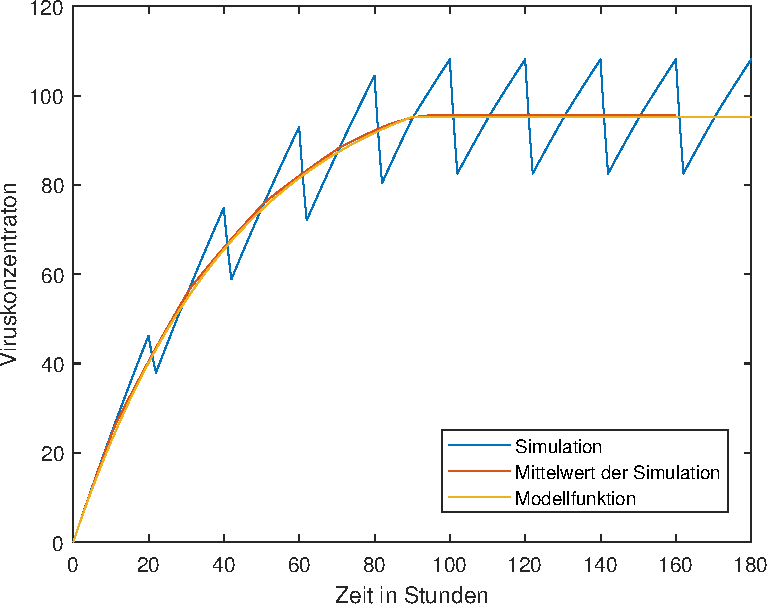
\includegraphics[width =0.8 \textwidth]{Simulation_fit1.pdf}
\caption{Vergleich der Modellfunktion mit der Simulation bei guter Raumlüftung}
\label{Abb: Modell gut}
\end{center}
\end{figure}

\begin{figure}[H]
\begin{center}
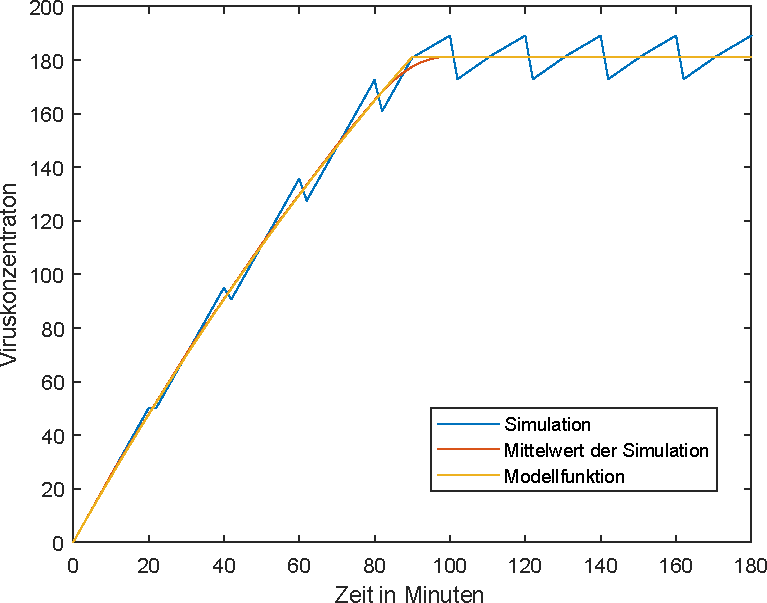
\includegraphics[width =0.8 \textwidth]{Simulation_fit2.pdf}
\caption{Vergleich der Modellfunktion mit der Simulation bei schlechter Raumlüftung}
\label{Abb: Modell schlecht}
\end{center}
\end{figure}

Durch Integration der Funktion lassen sich die aufgenommenen Partikel-Mengen bestimmen


\section{Bewertung der Einflussfaktoren}
Mit Hilfe von \autoref{Equ.: conc} lassen sich die einzelnen Einflussfaktoren sehr gut analysieren. Dabei lässt sich die Gleichung in 2 Teile zerlegen:
\begin{itemize}
\item Den Vorfaktor, der eine Streckung in y-Richtung erzeugt \\ ($a/b$)
\item Den exponentielle Teil, der die Zeit bis zum Erreichen des Maximums vorgibt \\ ($1 - exp(-b\cdot min(t,t\tief{vir}))$)
\end{itemize}
Daraus lässt sich ableiten:
\begin{itemize}
\item Steigt a, so steigt die Streckung in y-Richtung, was bedeutet, das die Viruskonzentration schneller anwächst und das Maximum höher liegt. Da a ein Maß für die ausgestoßene Menge an Partikeln bezogen auf die Raumgröße ist, ist dieses Verhalten auch durchaus plausibel.
\item Für b gilt das gleiche, jedoch befindet sich b auch im exponentiellen Teil der Gleichung. Durch eine Steigerung von b in diesem Bereich, erreicht der exponentiellen Teil schneller dem Wert von 1 und somit die Gesamtfunktion schneller die maximale Konzentration. Dieser Effekt ist dadurch zu erklären, dass sich durch die geringere maximale Konzentration schneller das Gleichgewicht zwischen Partikel-Bildung und Partikel-Abbau einstellen kann.
\end{itemize}
Zudem zeigt die Gleichung, dass Partikel-Abbau durch den Luftreiniger und Partikel-Abbau durch das Lüften sich sehr ähnlich verhalten. Diese Eigenschaft wird häufig in der Luftwechselrate $n$ zusammengefasst.
\begin{align}
n &=  \frac{\dot{V}}{V\tief{room}}
\end{align}
Mit \autoref{Equ.: konst b} lassen sich die beiden Lüftungseffekte als Luftwechselraten darstellen:
\begin{align}
n\tief{purifier} &= \frac{\dot{V}\tief{ap} \eta\tief{ap}}{V\tief{room}}\\
n\tief{vent} &= \frac{ \eta\tief{vent} }{t\tief{ventintervall}}\\
b = n\tief{purifier} + n\tief{vent}
\end{align}
In den folgenden Szenarien wird jeweils eine Größe variiert, während die anderen auf einem Standard-Wert verweilen. Die Standardwerte sind die folgenden:\\
\begin{tabular}{ll}
$t\tief{ges}$ & $\SI{5}{\hour}$   \\
$c\tief{breath}$ & $\SI{100}{particle\per\liter}$ \\   
$V\tief{breath}$ & $\SI{5}{\liter\per\minute}$   \\
$V\tief{room}$ & $\SI{200}{\cubic\meter}$   \\
$t\tief{vir}$ & $\SI{90}{\minute}$\\
$V\tief{ap}$ & $\SI{500}{\cubic\meter\per\hour}$   \\
$t\tief{ventintervall}$ & $\SI{20}{\minute}$    \\
\end{tabular}
\\ \\
Für Analysen zum Luftreiniger:\\
\begin{tabular}{ll}
$\eta\tief{vent}$ & $0.0$ \\
$\eta\tief{ap}$ & $0.95$    \\
\end{tabular}
\\ \\
Sonst:\\
\begin{tabular}{ll}
$\eta\tief{vent}$ & $0.5$ \\
$\eta\tief{ap}$ & $0.0$    \\
\end{tabular}

Da in den meisten Fällen entweder ein Luftreiniger läuft oder das Fenster geöffnet wird, wird in den folgenden Analysen jeweils die Effizienz der anderen Methode auf 0 gesetzt, so dass ihr Einfluss entfällt.\\
Da die meisten Schulen keine Luftfilter besitzen, wir 20 minütiges Lüften als Standard angenommen.\\
Die einzelnen Einflussfaktoren wurden immer mit $\frac{1}{4}$,$\frac{1}{2}$,$1$,$2$ und $4$ multipliziert, um vergleichbare Ergebnisse zu erhalten. Für die Werte der Effizienz würden jeweils sinnvolle Bereiche verwendet, da eine Effizienz über 1 nicht sinnvoll wäre.\\



\newpage
\subsection{Einfluss des Luftreinigers}








\begin{figure}[H]
\begin{center}
\includegraphics[width =1 \textwidth]{V_{ap}.eps}
\caption{Einfluss des Luftreiniger Volumenstroms (Faktor $b$)}
\label{Abb: lueftung}
\end{center}
\end{figure}


\begin{figure}[H]
\begin{center}
\includegraphics[width =1 \textwidth]{eta_{ap}.eps}
\caption{Einfluss der Luftreiniger Filtereffizienz (Faktor $b$)}
\label{Abb: lueftung}
\end{center}
\end{figure}

Bereits ein geringer Volumenstrom einer Luftreinigers bringt eine deutliche Verbesserung der Raumluft. Die Filtereffizienz hingegen hat nur einen sehr geringen Einfluss. Da mit steigender Filtereffizienz auch der Luftwiderstand und so der Energieverbrauch steigt, sollte eher ein Lüfter mit ineffizientem Filter gewählt werden.

\newpage
\subsection{Einfluss der Fensterlüftung}


\begin{figure}[H]
\begin{center}
\includegraphics[width =1 \textwidth]{t_{ventintervall}.eps}
\caption{Einfluss der Fensterlüftungsintervalle (Faktor $b$)}
\label{Abb: lueftung}
\end{center}
\end{figure}


\begin{figure}[H]
\begin{center}
\includegraphics[width =1 \textwidth]{eta_{vent}.eps}
\caption{Einfluss der Fensterlüftungseffizienz (Faktor $b$)}
\label{Abb: lueftung}
\end{center}
\end{figure}

Fensterlüftung kann aus Partikel-technischer Sicht durchaus mit Raumluftfiltern mithalten. Dafür muss die Raumluft jedoch ausreichend austauscht werden. Das heißt, das Durchzug oder ähnliche Bedingungen hergestellt werden müssen, damit die Luft auch im ausreichenden Maße ausgetauscht wird.

\newpage
\subsection{Einfluss der Aktivität}

\begin{figure}[H]
\begin{center}
\includegraphics[width =1 \textwidth]{c_{breath}.eps}
\caption{Einfluss der Atemkonzentration (Faktor $a$)}
\label{Abb: lueftung}
\end{center}
\end{figure}


\begin{figure}[H]
\begin{center}
\includegraphics[width =1 \textwidth]{V_{breath}.eps}
\caption{Einfluss der Atemmenge (Faktor $a$)}
\label{Abb: lueftung}
\end{center}
\end{figure}

Die Aktivität hat einen sehr hohen Einfluss auf das Infektionsrisiko. Die Atemmenge wirkt sich quadratisch auf die eingeatmete Partikelmenge aus, da sie die ausgestoßene und die eingeatmete Menge an partikelhaltiger Luft erhöht.


\newpage
\subsection{Einfluss der Viruslebensdauer}

\begin{figure}[H]
\begin{center}
\includegraphics[width =1 \textwidth]{t_{vir}.eps}
\caption{Einfluss der Viruslebensdauer}
\label{Abb: lueftung}
\end{center}
\end{figure}

Der Einfluss der Viruslebensdauer ist eher gering, solange sie größer als 90 Minuten ist. Sehr kurze Viruslebensdauern können jedoch das Infektionsrisiko deutlich senken.

\subsection{Einfluss der Raumgröße}

\begin{figure}[H]
\begin{center}
\includegraphics[width =1 \textwidth]{V_{room}.eps}
\caption{Einfluss der Raumgröße (Faktor $a$ und $b$)}
\label{Abb: lueftung}
\end{center}
\end{figure}

Die Raumgröße hat einen sehr signifikanten Einfluss. Verringert sie sich, verdünnt sich die ausgeatmete Luft nicht so stark, wodurch die Partikel-Konzentration in der Luft sehr stark ansteigt. Es ist jedoch zu beachten, das sich in größeren größeren Räumen meist mehr Personen aufhalten. Das erhöht die Chance, das eine oder mehrere Personen infiziert sind und es erhöht die Anzahl sich potentiell infizierender Personen.



\newpage
\RaggedRight
\bibliography{Bibliothek}


\listoffigures

\listoftables




\end{document}
